\documentclass[landscape,a4paper,12pt]{article}
\usepackage[margin=1.25cm]{geometry}
\usepackage{graphicx,xcolor,array,booktabs}
\usepackage[utf8]{inputenc}
\usepackage[T1]{fontenc}
\usepackage[brazil]{babel}
\pagestyle{empty}
\definecolor{navy}{HTML}{142D44}
\definecolor{teal}{HTML}{007F86}
\definecolor{pale}{HTML}{E8F3F3}
\definecolor{muted}{HTML}{486274}
\newcommand{\head}[4]{\par\noindent\hfill{\color{muted}\large #1 / 12}\par\vspace{.16cm}\noindent{\color{navy}\fontsize{26}{29}\selectfont\bfseries #2}\par\vspace{.22cm}\noindent{\color{teal}\rule{\textwidth}{1.1pt}}\par\vspace{.35cm}}
\newcommand{\foot}[3]{\par\vfill\noindent\colorbox{pale}{\parbox{\dimexpr\textwidth-2\fboxsep}{\color{navy}\bfseries #1\hfill\color{muted}#2\quad\textbar\quad #3}}\par}
\newcommand{\tagline}[1]{\par\vspace{.25cm}\noindent{\color{teal}\bfseries\large #1}\par}
\newcommand{\card}[2]{\colorbox{pale}{\parbox[t]{#1}{\vspace{.15cm}\color{navy}#2\vspace{.15cm}}}}
\begin{document}
\head{1}{Triagem assistida de radiografias de tórax}{}{}
\vspace{.4cm}
\begin{minipage}[t]{.57\textwidth}\vspace{0pt}
{\color{navy}\fontsize{22}{27}\selectfont Uma fila de leitura pode priorizar exames com maior probabilidade de alteração.}\par\vspace{.75cm}
{\color{teal}\Large\bfseries Pergunta do projeto}\par\vspace{.15cm}
{\Large Como apoiar essa priorização sem transformar o modelo em diagnóstico?}\par\vspace{.65cm}
{\color{muted}\large Protótipo acadêmico com radiografias públicas. A decisão clínica permanece com profissionais.}
\end{minipage}\hfill
\begin{minipage}[t]{.37\textwidth}\vspace{0pt}\card{.94\linewidth}{\centering\Large\bfseries 5.606 imagens\\[.35cm]\large NIH ChestX-ray14\\[.55cm]\Large\bfseries 2 classes\\[.2cm]\large NORMAL / ALTERADA} \end{minipage}
\foot{Lucas Bonissoni}{0:40}{Problema}\newpage
\head{2}{O produto organiza prioridades, não laudos}{}{}
\vspace{.35cm}
\begin{center}\card{.24\textwidth}{\centering\Large Radiografia\\[.2cm]\normalsize entrada 224 $\times$ 224}\quad{\color{teal}\LARGE$\longrightarrow$}\quad\card{.24\textwidth}{\centering\Large ResNet-50\\[.2cm]\normalsize probabilidade ALTERADA}\quad{\color{teal}\LARGE$\longrightarrow$}\quad\card{.24\textwidth}{\centering\Large Fila de leitura\\[.2cm]\normalsize prioridade / revisão}\end{center}
\vspace{.6cm}\large\color{navy}
A saída distingue \textbf{prioridade alta}, \textbf{média}, \textbf{rotina} e uma faixa \textbf{indeterminada}. Uma checagem de qualidade pode sinalizar imagem inadequada.\par\vspace{.4cm}
\tagline{A fila pode ajudar a ordenar. Ela não identifica a doença nem dispensa o radiologista.}
\foot{Lucas Bonissoni}{0:40}{Fluxo de triagem}\newpage
\head{3}{Dados e rótulos usados no experimento}{}{}
\begin{minipage}[t]{.50\textwidth}\vspace{0pt}
{\color{navy}\Large Fonte: amostra pública do NIH ChestX-ray14.}\par\vspace{.45cm}
\card{.94\linewidth}{\Large\bfseries NORMAL\par\normalsize rótulo original \emph{No Finding}}\par\vspace{.35cm}
\card{.94\linewidth}{\Large\bfseries ALTERADA\par\normalsize qualquer outro achado registrado}\par\vspace{.45cm}
{\color{muted}\large Rótulos extraídos de laudos, sem revisão clínica neste projeto.}
\end{minipage}\hfill
\begin{minipage}[t]{.42\textwidth}\vspace{0pt}
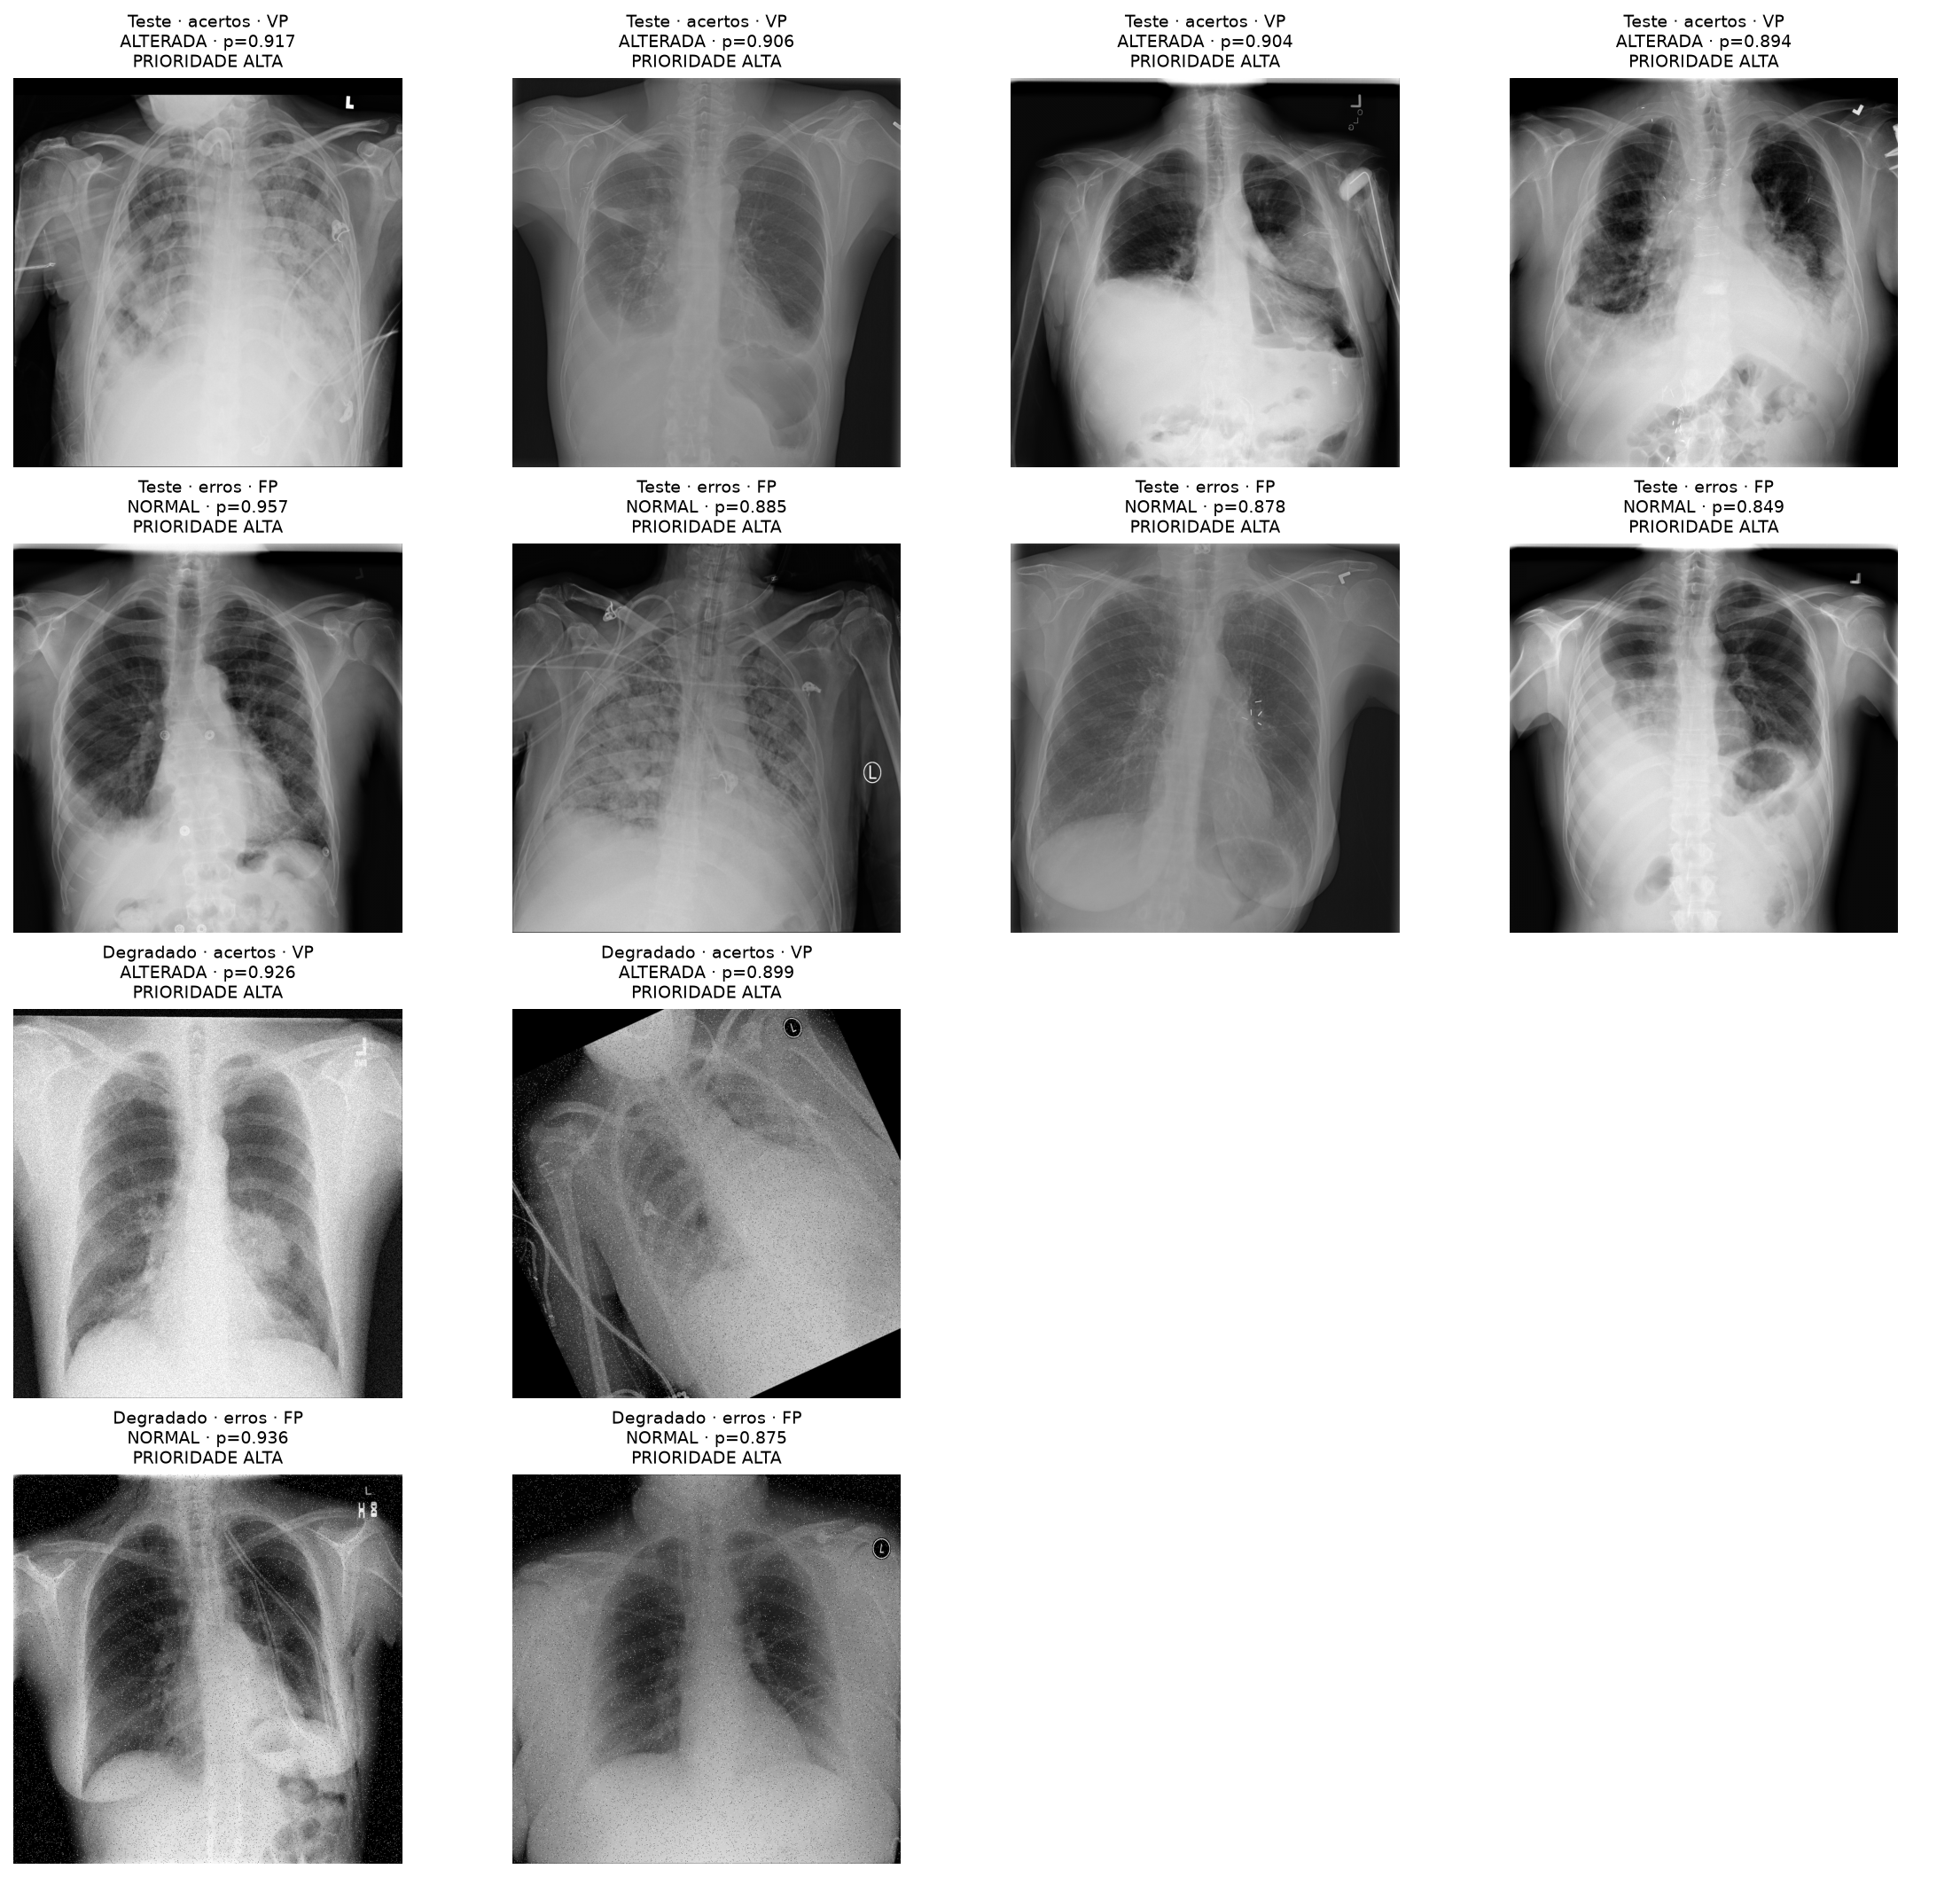
\includegraphics[width=\linewidth,height=8.1cm,keepaspectratio]{../artigo/figuras/acertos_erros.png}\par\small Exemplos de radiografias e previsões no teste.
\end{minipage}
\foot{Luiz Cenci}{0:40}{Dataset}\newpage
\head{4}{A separação por paciente protege o teste}{}{}
\vspace{.25cm}
\begin{center}
\card{.28\textwidth}{\centering\color{teal}\fontsize{25}{28}\selectfont\bfseries 3.931\par\color{navy}\Large treino}\quad
\card{.28\textwidth}{\centering\color{teal}\fontsize{25}{28}\selectfont\bfseries 531\par\color{navy}\Large validação}\quad
\card{.28\textwidth}{\centering\color{teal}\fontsize{25}{28}\selectfont\bfseries 1.144\par\color{navy}\Large teste}
\end{center}
\vspace{.9cm}
{\color{navy}\Large Pacientes exclusivos em cada divisão. Limiares e limites de qualidade foram ajustados na validação; métricas finais usam o teste isolado.}\par\vspace{.65cm}
\tagline{Total: 5.606 imagens. O resultado mede esse recorte público, não uma população clínica externa.}
\foot{Luiz Cenci}{0:40}{Protocolo}\newpage
\head{5}{Modelo: transferência de aprendizado}{}{}
\begin{minipage}[t]{.46\textwidth}\vspace{0pt}
{\color{navy}\Large ResNet-50 com pesos ImageNet.}\par\vspace{.4cm}
\large Radiografias em cinza: 224 $\times$ 224 pixels e três canais.\par\vspace{.35cm}
Treino em duas fases: base congelada; depois, ajuste fino do último bloco convolucional.\par\vspace{.35cm}
Ponderação de classes e aumentos de rotação, zoom e contraste.\par\vspace{.5cm}
{\color{muted}Comparação: CNN baseline treinada do zero.}
\end{minipage}\hfill
\begin{minipage}[t]{.45\textwidth}\vspace{0pt}
\card{.95\linewidth}{\Large\bfseries Entrada\par\normalsize radiografia normalizada}\par\vspace{.3cm}
\card{.95\linewidth}{\Large\bfseries Base visual\par\normalsize ResNet-50 pré-treinada}\par\vspace{.3cm}
\card{.95\linewidth}{\Large\bfseries Saída\par\normalsize probabilidade de ALTERADA}
\end{minipage}
\foot{Mauro Cella}{0:40}{Treinamento}\newpage
\head{6}{A probabilidade vira uma decisão de fila}{}{}
\vspace{.15cm}
\begin{center}
\card{.27\textwidth}{\centering\Large\bfseries 0,231\par\normalsize limiar de rotina}\quad
\card{.27\textwidth}{\centering\Large\bfseries $\pm$ 0,05\par\normalsize faixa indeterminada}\quad
\card{.27\textwidth}{\centering\Large\bfseries 0,788\par\normalsize prioridade alta}
\end{center}
\vspace{.75cm}
\begin{minipage}[t]{.48\textwidth}\vspace{0pt}{\color{navy}\Large Limiar baixo favorece o recall de exames ALTERADA. O custo é elevar falsos positivos.}\end{minipage}\hfill
\begin{minipage}[t]{.45\textwidth}\vspace{0pt}{\color{navy}\Large Antes da prioridade, contraste e nitidez são comparados a limites calibrados na validação.}\end{minipage}
\vspace{.6cm}\tagline{A checagem atual não cobre todas as falhas de qualidade.}
\foot{Mauro Cella}{0:40}{Camada de decisão}\newpage
\head{7}{No teste, a ResNet-50 supera o baseline}{}{}
\vspace{.2cm}
{\large\color{navy}\begin{center}\renewcommand{\arraystretch}{1.6}
\begin{tabular}{lcc}
\toprule
Métrica no teste de 1.144 imagens & Baseline & ResNet-50\\
\midrule
Recall & 85,5\% & \textbf{90,4\%}\\
Precisão & 48,4\% & \textbf{54,3\%}\\
F1 & 61,8\% & \textbf{67,8\%}\\
Balanced accuracy & 53,5\% & \textbf{62,4\%}\\
AUROC & 53,7\% & \textbf{72,5\%}\\
\bottomrule
\end{tabular}\end{center}}
\vspace{.3cm}\tagline{Recall foi priorizado porque um falso negativo pode permanecer na rotina.}
\foot{Matheus de Aquino}{0:40}{Métricas gerais}\newpage
\head{8}{O ganho em recall tem um custo}{}{}
\begin{minipage}[t]{.47\textwidth}\vspace{0pt}
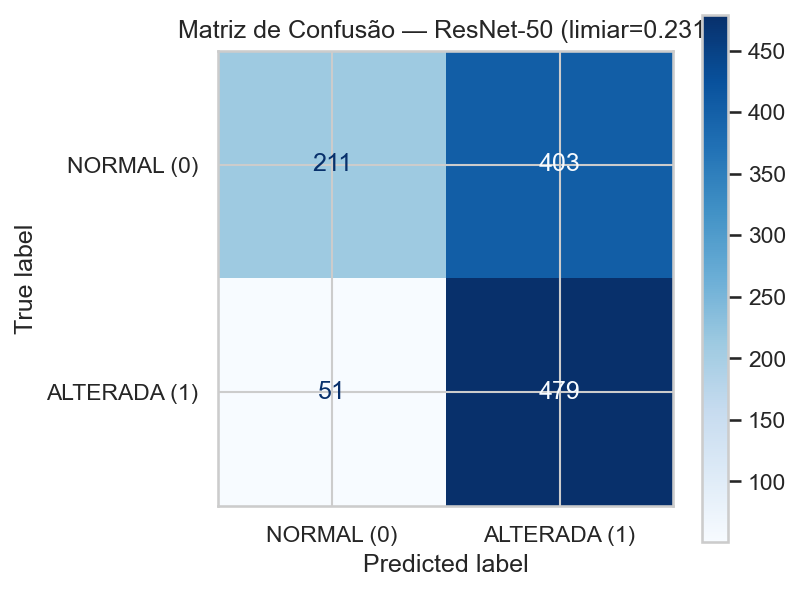
\includegraphics[width=\linewidth,height=8.0cm,keepaspectratio]{../artigo/figuras/confusao_resnet50.png}\par\small Matriz de confusão no teste.
\end{minipage}\hfill
\begin{minipage}[t]{.45\textwidth}\vspace{0pt}
{\color{navy}\Large 479 verdadeiros positivos\par 51 falsos negativos\par 403 falsos positivos\par 211 verdadeiros negativos}\par\vspace{.55cm}
{\color{teal}\large\bfseries Distribuição da fila}\par\vspace{.1cm}
{\large Alta 44; média 725; indeterminada 188; rotina 187.}\par\vspace{.35cm}
{\color{navy}\large 34 das 187 imagens em rotina tinham rótulo ALTERADA.}
\end{minipage}
\foot{Matheus de Aquino}{0:40}{Erros e prioridades}\newpage
\head{9}{Teste de robustez: pares originais e degradados}{}{}
\begin{minipage}[t]{.43\textwidth}\vspace{0pt}
{\color{navy}\Large 150 radiografias do teste: 75 NORMAL e 75 ALTERADA.}\par\vspace{.45cm}
\large Cada imagem tem uma versão degradada. Foram aplicados cinco tipos, 30 imagens por tipo:\par\vspace{.2cm}
{\color{teal}\large\bfseries ruído, rotação, corte, baixo contraste e combinação.}\par\vspace{.55cm}
{\color{muted}\large A comparação usa o mesmo limiar nas duas versões.}
\end{minipage}\hfill
\begin{minipage}[t]{.52\textwidth}\vspace{0pt}
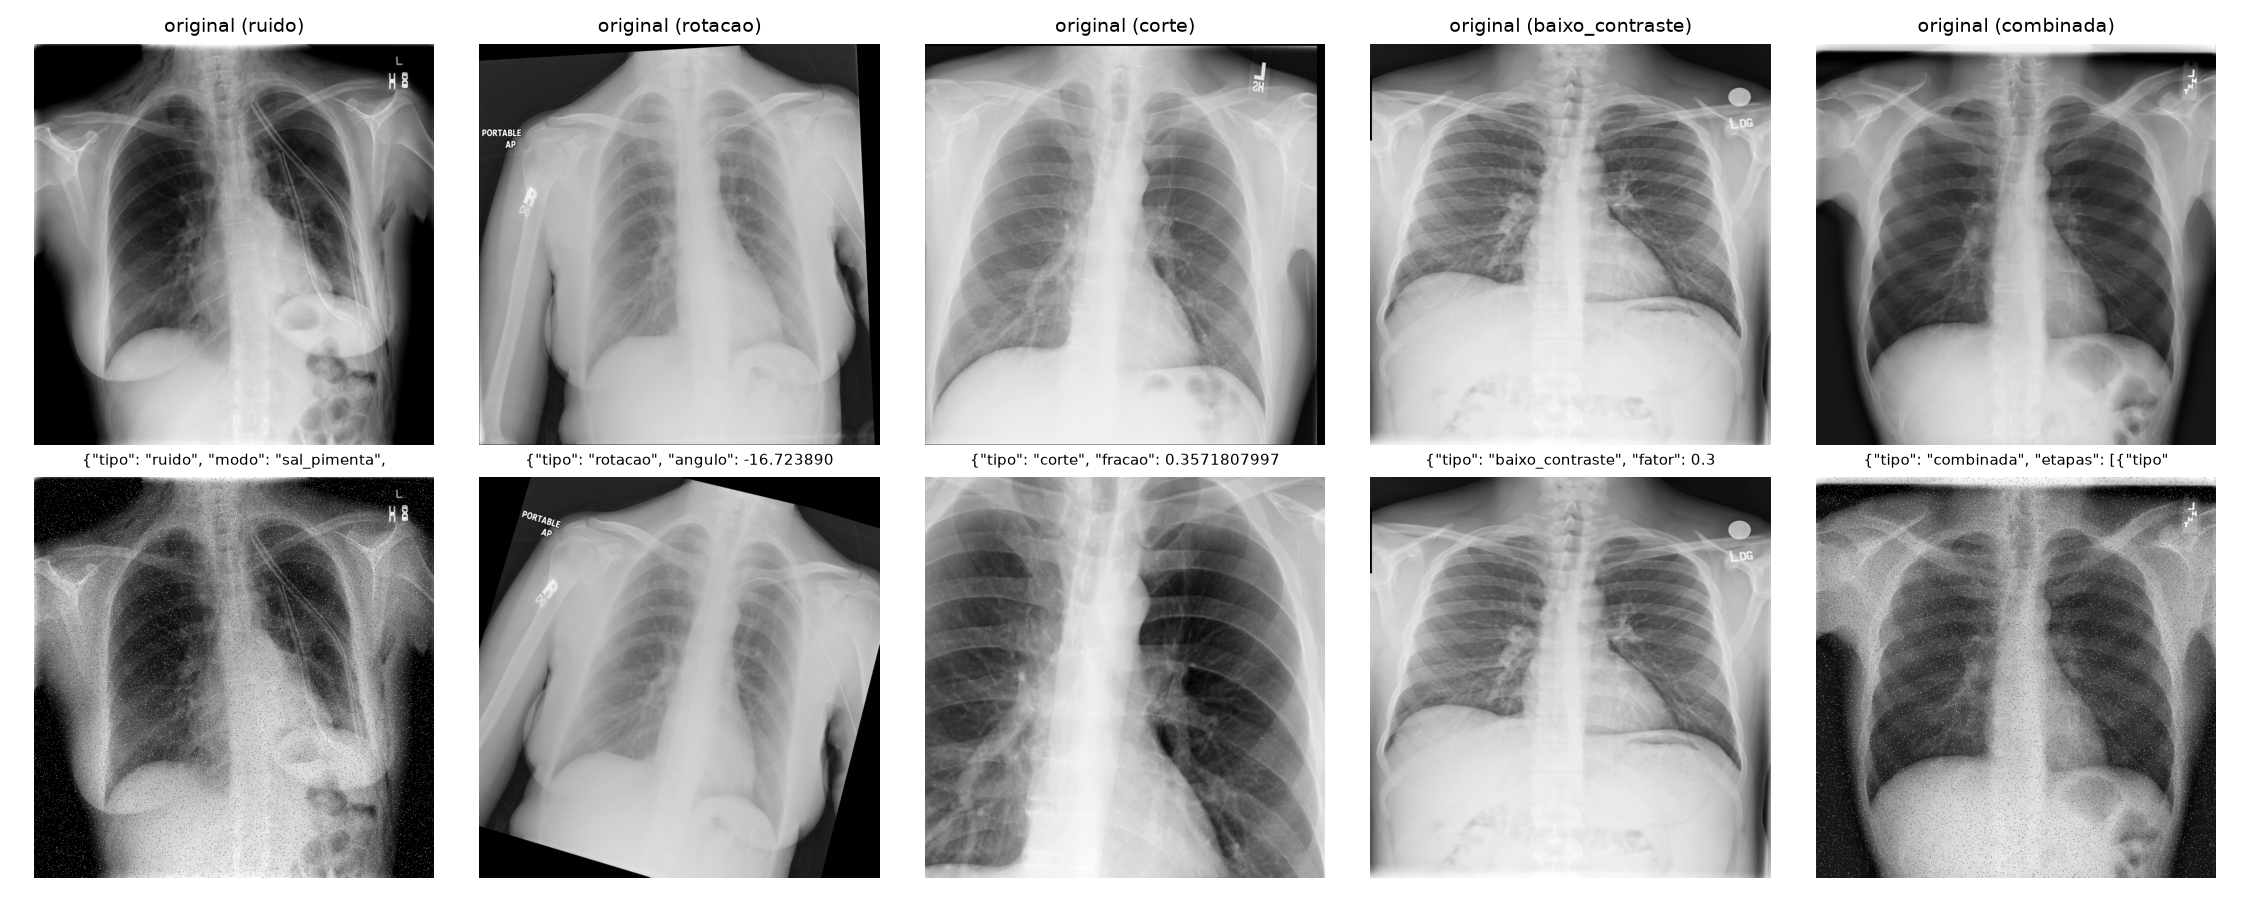
\includegraphics[width=\linewidth,height=8.0cm,keepaspectratio]{../artigo/figuras/degradado_exemplos.png}\par\small Exemplos sintéticos produzidos para o experimento.
\end{minipage}
\foot{Murilo Ghizzi}{0:40}{Conjunto degradado}\newpage
\head{10}{A degradação reduziu o equilíbrio dos acertos}{}{}
\begin{minipage}[t]{.47\textwidth}\vspace{0pt}
{\color{navy}\large\bfseries Comparação pareada de 150 imagens}\par\vspace{.3cm}
{\large\color{navy}Balanced accuracy: \textbf{0,600 $\rightarrow$ 0,520}\par F1: \textbf{0,688 $\rightarrow$ 0,654}\par Recall: \textbf{0,880 $\rightarrow$ 0,907}\par Falsos positivos: \textbf{51 $\rightarrow$ 65}}\par\vspace{.45cm}
{\color{teal}\large Mais recall não significa melhora geral: a precisão caiu de 0,564 para 0,511.}\par\vspace{.3cm}
{\color{muted}\normalsize A checagem sinalizou 30/30 casos de baixo contraste e corte, mas nenhum de rotação ou ruído.}
\end{minipage}\hfill
\begin{minipage}[t]{.47\textwidth}\vspace{0pt}
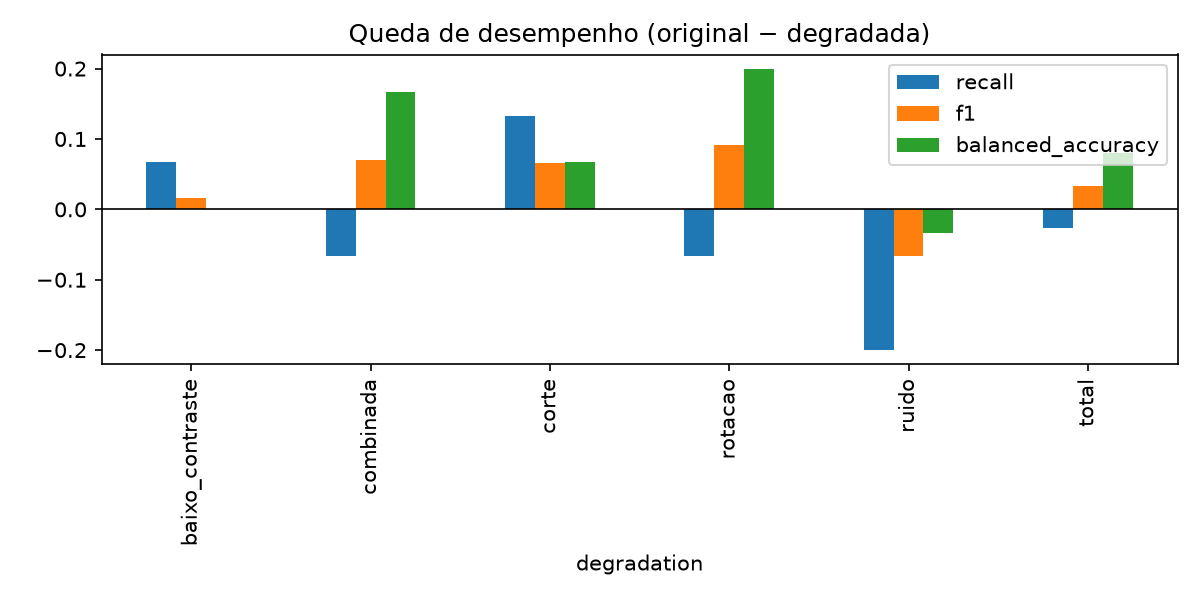
\includegraphics[width=\linewidth,height=8.0cm,keepaspectratio]{../artigo/figuras/degradado_queda.png}
\end{minipage}
\foot{Murilo Ghizzi}{0:40}{Robustez}\newpage
\head{11}{Grad-CAM ajuda a inspecionar erros}{}{}
\begin{minipage}[t]{.42\textwidth}\vspace{0pt}
{\color{navy}\Large Foram inspecionados 15 casos: 12 do teste e 3 degradados.}\par\vspace{.45cm}
\large Nos três falsos negativos selecionados do teste, o foco principal ficou \textbf{fora dos pulmões}.\par\vspace{.5cm}
{\color{teal}\large O mapa mostra regiões associadas à previsão, não uma explicação clínica causal.}\par\vspace{.4cm}
{\color{muted}\normalsize Não generalizar essa observação para todos os erros.}
\end{minipage}\hfill
\begin{minipage}[t]{.53\textwidth}\vspace{0pt}
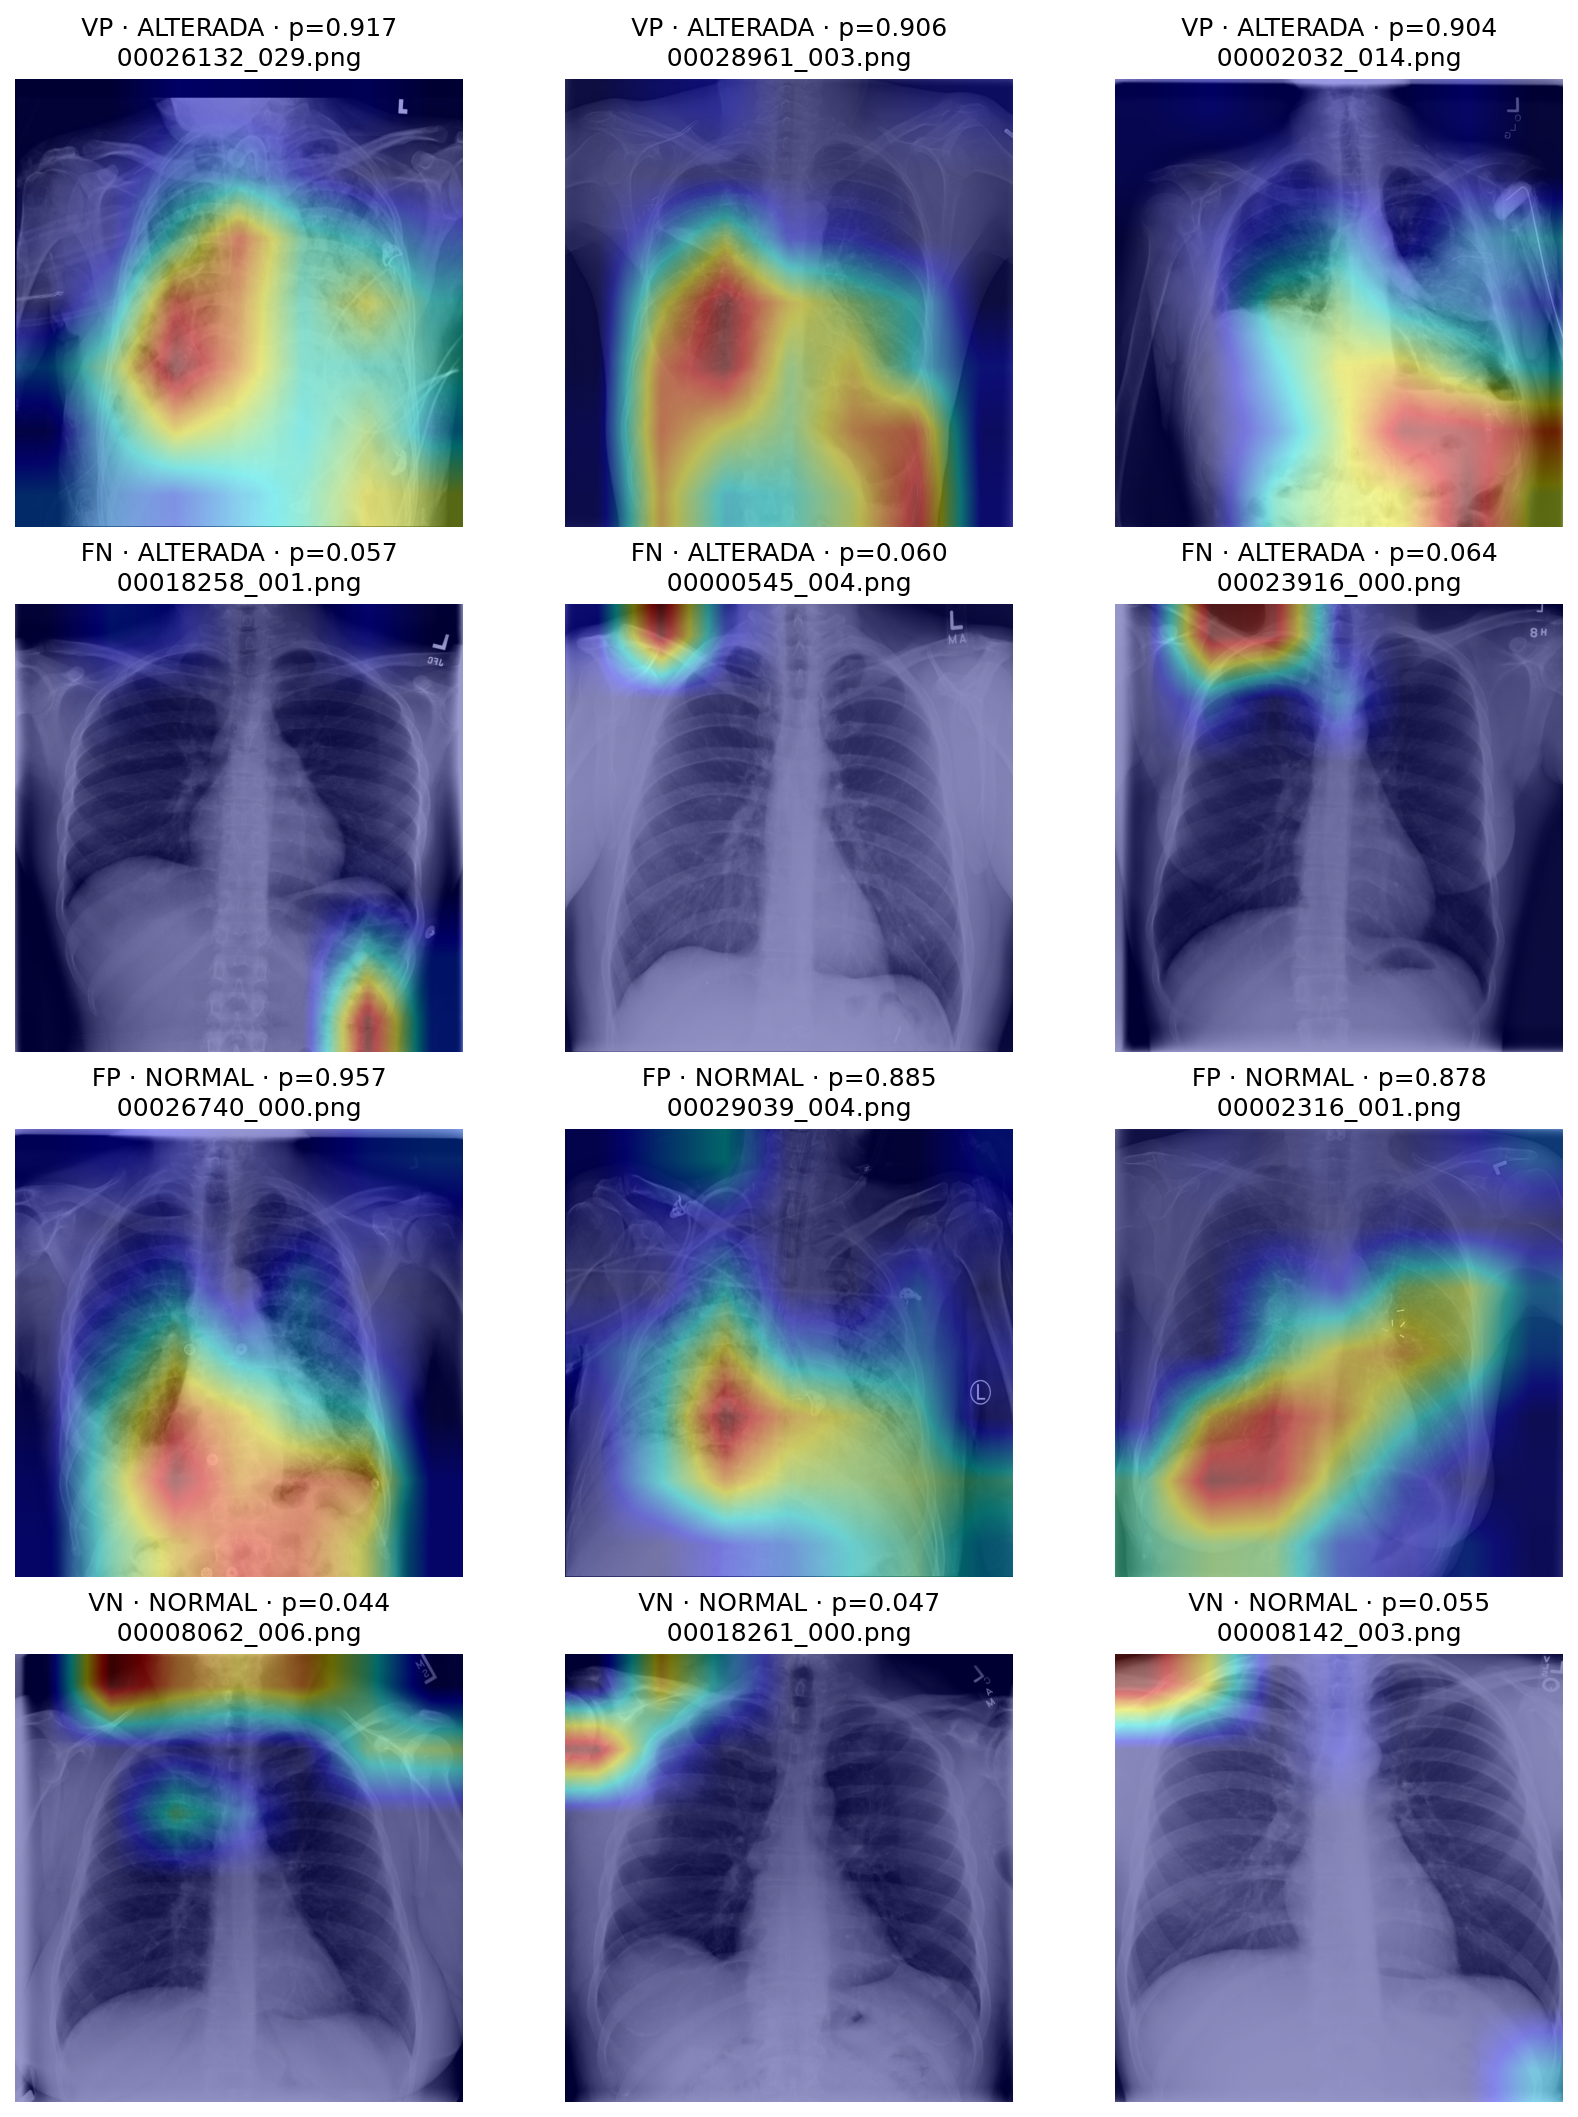
\includegraphics[width=\linewidth,height=8.1cm,keepaspectratio]{../artigo/figuras/gradcam_teste.png}\par\small Casos selecionados, organizados por acerto e erro.
\end{minipage}
\foot{Alana Kunrath}{0:40}{Interpretabilidade}\newpage
\head{12}{Conclusão e limites do protótipo}{}{}
\vspace{.2cm}
\begin{minipage}[t]{.46\textwidth}\vspace{0pt}
{\color{teal}\Large\bfseries O que aprendemos}\par\vspace{.25cm}
{\color{navy}\large A ResNet-50 melhorou as métricas frente ao baseline, mas produziu 51 falsos negativos e 403 falsos positivos no teste.}\par\vspace{.45cm}
{\color{navy}\large Sob degradação, a balanced accuracy caiu. A checagem de qualidade tem lacunas.}
\end{minipage}\hfill
\begin{minipage}[t]{.46\textwidth}\vspace{0pt}
{\color{teal}\Large\bfseries Antes de qualquer uso clínico}\par\vspace{.25cm}
{\color{navy}\large Validar em dados externos e com rótulos revisados. Melhorar calibração e detecção de rotação, ruído e cortes. Avaliar impacto real na fila de leitura.}\par\vspace{.45cm}
{\color{muted}\large A alternativa de imagens degradadas precisa de concordância do professor para a disciplina.}
\end{minipage}
\vspace{.55cm}\tagline{Conclusão: apoio experimental à triagem, nunca diagnóstico automático.}
\foot{Alana Kunrath}{0:40}{Encerramento}
\end{document}
